\documentclass[../mathNotesPreamble]{subfiles}

\begin{document}
%  \relscale{1.4} %TODO
  \section{3.3: The Chain Rule}
  \begin{ex*}
    Let $f(x)=\parens{x^3+x+1}^2$. Find $f'(x)$
    \begin{extasks}[after-item-skip=\stretch{1}](1)
      \task using the product rule
      \task by expanding 
    \end{extasks}
  \end{ex*}
  \vspace*{\stretch{1}}
  What about $\displaystyle\ddx\sbrkt{\parens{x^3+x+1}^{100}}$?
  \pagebreak

  \noindent\textbf{Composite Functions:}

  \begin{thmBox*}
    Let $f$ and $g$ be functions of $x$. Then, the \textbf{composite functions} $g$ of $f$ (denoted $g\circ f$) and $f$ of $g$ (denoted $f\circ g$) are defined as:
    \begin{align*}
      (g\circ f)(x)&=g\parens{f(x)}\\
      (f\circ g)(x)&=f\parens{g(x)}
    \end{align*}
  \end{thmBox*}
  \begin{ex*}
    'Break-down' the following composite functions:
  \end{ex*}
  \begin{extasks}[after-item-skip=\stretch{1}](2)
    \task $\dfrac{1}{x+3}$
    \task $\parens{x^4+3x-8}^3$
    \task $\parens{\dfrac{1-x}{x^3+1}}^4$
    \task $\dfrac{3x}{\sqrt{(x+1)^2-1}}$
  \end{extasks}
  \vspace*{\stretch{1}}
  \pagebreak
  
  \begin{thmBox*}[Rule 7: The Chain Rule]
    \begin{align*}
      \ddx\sbrkt{f\parens{g(x)}}&=f'\parens{g(x)}g'(x)
    \end{align*}
    If $y=f(u)$ and $u=g(x)$, then
    \begin{align*}
      \dydx&=\dfrac{dy}{du}\cdot\dfrac{du}{dx}
    \end{align*}
  \end{thmBox*}
  
  \noindent
  {\centering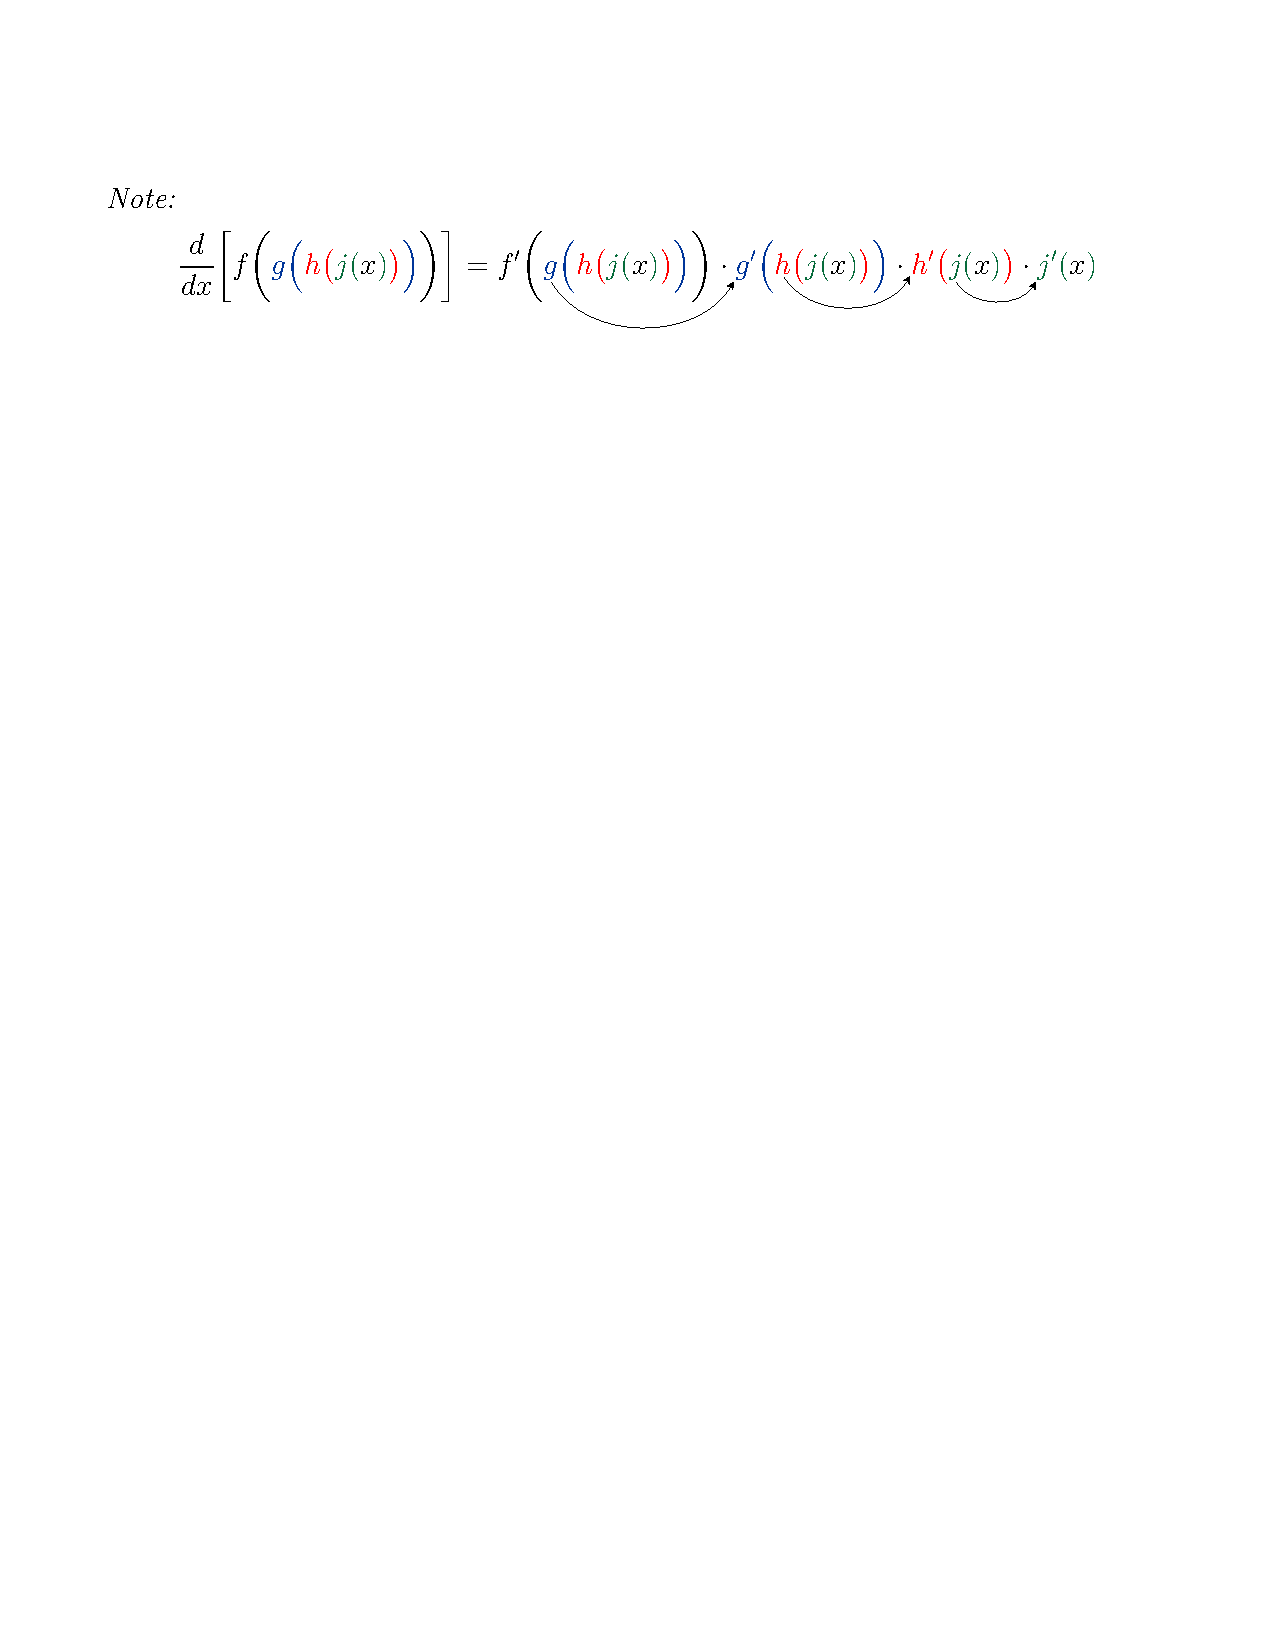
\includegraphics[width=\textwidth, clip, trim=0.5in 220mm 0.5in 20mm]{chain_rule_ex}}
  
%\newcommand{\tikzmark}[2]{%
%  \tikz[baseline=(#1.base), remember picture]%
%  \node[inner sep=0pt] (#1)%
%  {\ensuremath{#2}};%
%}
%
%  \emph{Note:}
%  % f black              \bigg
%  % g lander_blue        \Big
%  % h red                \big
%  % j lander_FrontLawn
%  \begin{align*}
%    \ddx\sbrkt{
%      \textcolor{black}{f\bigg(}
%        \textcolor{lander_blue}{g\Big(}
%          \textcolor{red}{h\big(}
%            \textcolor{lander_FrontLawn}{j(}
%              x
%            \textcolor{lander_FrontLawn}{)}
%          \textcolor{red}{\big)}
%        \textcolor{lander_blue}{\Big)}
%      \textcolor{black}{\bigg)}
%      }
%      &=\textcolor{black}{f'\bigg(}
%        \textcolor{lander_blue}{\tikzmark{g}{g}\Big(}
%          \textcolor{red}{h\big(}
%            \textcolor{lander_FrontLawn}{j(}
%              x
%            \textcolor{lander_FrontLawn}{)}
%          \textcolor{red}{\big)}
%        \textcolor{lander_blue}{\Big)}
%      \textcolor{black}{\bigg)}
%      \cdot
%      \textcolor{lander_blue}{\tikzmark{gp}{g}'\Big(}
%        \textcolor{red}{\tikzmark{h}{h}\big(}
%          \textcolor{lander_FrontLawn}{j(}
%            x
%          \textcolor{lander_FrontLawn}{)}
%        \textcolor{red}{\big)}
%      \textcolor{lander_blue}{\Big)}
%      \cdot
%      \textcolor{red}{\tikzmark{hp}{h}'\big(}
%        \textcolor{lander_FrontLawn}{\tikzmark{j}{j}(}
%          x
%        \textcolor{lander_FrontLawn}{)}
%      \textcolor{red}{\big)}
%      \cdot
%      \textcolor{lander_FrontLawn}{\tikzmark{jp}{j}'(}
%        x
%      \textcolor{lander_FrontLawn}{)}
%  \end{align*}
%  \begin{tikzpicture}[overlay, remember picture,
%    myArrow/.style={->, in=-120, out=-60, shorten >=1pt, shorten <=1pt}]
%    \draw[myArrow] (g.south) to (gp.south west);
%    \draw[myArrow] (h.south) to (hp.south west);
%    \draw[myArrow] (j.south) to (jp.south west);
%  \end{tikzpicture}
  \begin{thmBox*}[The General Power Rule]
    \begin{align*}
      \ddx\sbrkt{\parens{f(x)}^n}&=n\parens{f(x)}^\nmo f'(x)
    \end{align*}
  \end{thmBox*}
  \pagebreak
  
  \begin{ex*}
    Find the derivative of the following functions
  \end{ex*}
  \begin{extasks}[after-item-skip=\stretch{1}](1)
    \task $F(x)=\parens{x^3+x+1}^{100}$
    \task $G(t)=\parens{3x+1}^2$
    \task $H(u)=\sqrt{u^2+1}-3$
    \task $J(\nu)=\nu^2\parens{2\nu+3}^5$
  \end{extasks}
  \vspace*{\stretch{1}}
  \pagebreak
  
  \begin{extasks}[after-item-skip=\stretch{1}](1)
    \task $\kappa(x)=\parens{2x^2+3}^4\parens{3x-1}^5$
    \task $\tau(x)=\dfrac{1}{\parens{4x^2-7}^2}$
  \end{extasks}
  \vspace*{\stretch{1}}
  \begin{ex*}
    Find the equation of the line tangent to $f(x)$ at $\parens{0,\dfrac{1}{8}}$
    \begin{align*}
      f(x)=\parens{\dfrac{2x+1}{3x+2}}^3
    \end{align*}
  \end{ex*}
  \pagebreak
  
  \begin{ex*}
    The membership of The Fitness Center, which opened a few years ago, is approximated by the function
    \begin{align*}
      N(t)=100\parens{64+4t}^{2/3} \qquad \parens{0\leq t\leq 52}
    \end{align*}
    where $N(t)$ gives the number of members at the beginning of week $t$.
  \end{ex*}
  \begin{extasks}[after-item-skip=\stretch{1}](1)
    \task Find $N'(t)$
    \task How fast was the center's membership increasing initially $(t=0)$?
    \task How fast was the membership increasing at the beginning of the 40th week?
    \task What was the membership when the center first opened? At the beginning of the 40th week?
  \end{extasks}
  \vspace*{\stretch{1}}
  \pagebreak

  \begin{thmBox*}[Rule 1: Derivative of a Constant]
    \vspace*{-\baselineskip}
    \begin{align*}
        \ddx\sbrkt{c}&=0\\[15pt]
      \intertext{\textbf{Rule 2: The Power Rule}}
        \ddx\sbrkt{x^n}&=nx^\nmo\\[15pt]
      \intertext{\textbf{Rule 3: Derivative of a Constant Multiple of a Function}}
        \ddx\sbrkt{cf(x)}&=c\ddx\sbrkt{f(x)}\\[15pt]
      \intertext{\textbf{Rule 4: The Sum Rule}}
        \ddx\sbrkt{f(x)\pm g(x)}&=\ddx\sbrkt{f(x)}\pm \ddx\sbrkt{g(x)}\\[15pt]
      \intertext{\textbf{Rule 5: The Product Rule}}
        \ddx\sbrkt{f(x)\cdot g(x)}&=f'(x)\cdot g(x)+f(x)\cdot g'(x)\\[15pt]
      \intertext{\textbf{Rule 6: The Quotient Rule}}
        \ddx\sbrkt{\dfrac{f(x)}{g(x)}}&=\dfrac{g(x)f'(x)-f(x)g'(x)}{\sbrkt{g(x)}^2}\\[15pt]
      \intertext{\textbf{Rule 7: The Chain Rule}}
        \ddx\sbrkt{f\parens{g(x)}}&=f'\parens{g(x)}g'(x)
    \end{align*}
  \end{thmBox*}
  \pagebreak
\end{document}
